%%%%%%%%%%%%%%%%%%%%%%%%%%%%%%%%%%%%%%%%%%%%%%%%%%%%%%%%%%%%%%%%%%%%%%
%
%   File          : related_work.tex
%   Author(s)     : Ashwin Shashidharan <ashashi3@ncsu.edu> and Jitesh Shah <jhshah@ncsu.edu>
%   Description   : Related Work for the Project
%
%   Last Modified : Wed Sep 28 21:30:30 EDT 2011
%   By            :  Ashwin Shashidharan <ashashi3@ncsu.edu> and Jitesh Shah <jhshah@ncsu.edu>
%
%%%%%%%%%%%%%%%%%%%%%%%%%%%%%%%%%%%%%%%%%%%%%%%%%%%%%%%%%%%%%%%%%%%%%%

\documentclass[10pt,twocolumn,pdftex]{article}
\usepackage[margin=1in]{geometry}
\usepackage{comment}
\usepackage{ifthen}
\usepackage{graphicx}
\usepackage[hyphens]{url}
\usepackage{times}
% hyperref sometimes causes strange build errors. Comment if problems
\usepackage[pdftex,colorlinks=true,citecolor=black,filecolor=black,%
            linkcolor=black,urlcolor=black,draft]{hyperref}
%\usepackage{listings}
%\usepackage{fancyvrb}
%\usepackage{amsmath}
%\usepackage{amsthm}
%\usepackage{amssymb}

% Some quick utils
% Use:
% \begin{itemize} \itembase{3pt}
%  \item ...
% \end {itemize}
\newcommand{\itembase}[1]{\setlength{\itemsep}{#1}}

\title{Enabling Cloud Customers to Trust the Cloud}

\author{Ashwin Shashidharan and Jitesh Shah \\
\url{{ashashi3,jhshah}@ncsu.edu}
}
\date{November 30, 2011}
\begin{document}

\maketitle

\begin{abstract}
Cloud computing has emerged into a very popular \cite{adoption-survey} means of scaling up quickly without the associated infrastructure costs. The promise is complete freedom from maintaining own server infrastructures and moving to third-party infrastructure providers. Despite it's increasing popularity, a significant chunk of applications haven't yet found a place in the cloud. The reason is the lack of guarantees, from the cloud provider, about the security of customer data stored on the cloud. Even in the presence of such guarantees, the cloud customer would want to ensure that a very small chunk of \emph{auditable} infrastructure on the cloud side is trusted. Using that as a Trust Computing Base (TCB), the customer would build his own security to protect his data, thus, having the guarantees. Note that the threat to the customer data does \emph{not} come from the cloud provider, but, attacks on the cloud provider by competitors using the same cloud service or other external attackers. 

This paper proposes a way to enable the customer to protect its data in the face of a cloud compromise. Two key technologies are used to build the security architecture: SELinux (Security Enhanced Linux) \cite{SELinux} and TPM (Trusted Platform Modules) \cite{TCG}. Both of these technologies allow confining the root user. We also describe a range of feasible attacks and how the customer data can be protected in the face on these attacks using the proposed architecture.\\ \\
\emph{Keywords}:  Trusting the cloud, SELinux, TPM, SSL/TLS, symmetric encryption/integrity verification.
\end{abstract}

\section{Introduction}
According to a Berkeley publication \cite{controlling-data-in-the-cloud}, all the top five software companies by sales revenue have their own cloud offerings. Popular sites such as reddit.com and quora.com run completely off the cloud. Merrill Lynch estimates the market capitalization of the "Cloud Computing" sector to be as large as 16B in 2011. Inspite of such impressive growth, a Morgan-Stanley survey \cite{morgan-stanley} says that only 28\% respondents of the survey use public cloud of some form in their daily operations whereas only 14\% use IaaS services of any kind. Various publications \cite{controlling-data-in-the-cloud, ENISA} clearly identify the risks associated with security of the storing data in the cloud. Fear of leakage of sensitive data from the cloud is a common thread in these publications. These risks induce a "Fear of the Cloud", thus, slowing down adoption. Vulnerabilities discovered in popular cloud services like Amazon EC2 \cite{amazon-ec2-vulnerability} and Dropbox \cite{dropbox-vulnerability} exacerbates the fear. 

For corporations to offload their secure data to the cloud, they need to have guarantees against leakage of thire data. Such guarantees can come only from a huge audit of the cloud provider, which might be unfeasible and time consuming considering the size of the cloud providers, or getting themselves involved in designing of the security on the cloud provider side. The cloud can thus be viewed, from the perspective of our project, as a provider of infrastructure and a Trusted Computing Base (TCB) which can be utilized by the cloud customers to enforce a security policy. \\

Various methods have been proposed in the past to avoid data leakage from the cloud. Simply encrypting data in the cloud (without any trusted software) has been discussed in literature sparingly \cite{cryptographic-cloud-storage, towards-secure-cloud-storage}. The problem with just encrypting the data, without attestation of the underlying software, is that the underlying software could have been maliciously modified by an attacker who has broken into the cloud provider. A modified guest kernel would definitely be able to steal all the encryption keys. So, even though encryption is an essential component of securing the data, a trusted computing base is essential too.

Setting up a Trusted Computing Base (TCB) for the cloud has been more widely discussed \cite{towards-trusted-cloud-computing, seeding-clouds-with-trust-anchors, terra, semantic-remote}. A TCB is setup with an established root of trust. The root of trust is usually a TPM (Trusted Platform Module). Beginning with the TPM, the BIOS, bootloader and the Operating System are verified before passing control to them. Any modification to any of the above components would lead to failure of Remote Attestation. The problem with such an approach is that, it provides security only in static aspects. Any attack on the runtime system (process, memory, etc) would go undetected. 

Literature also talks about runtime integrity verification \cite{integrity-1, integrity-2, integrity-3, integrity-4}. The problem with runtime integrity verification is that they are very difficult to get right in practice. No cloud in the current market offers runtime integrity verification \cite{seeding-clouds-with-trust-anchors}.

Without runtime integrity protection, the data on the cloud will still be vulnerable to attacks of the dynamic nature. A practical alternative to runtime integrity verification is to sandbox the trusted VM launcher process, minimize its interaction with the outside world and audit the small external facing code thoroughly for security vulnerabilities. Thus, in addition to encryption and trusted computing, we propose to use strong Mandatory Access Control (MAC) based confinement techniques to sandbox the trusted VM launcher and the kernel images. This can be viewed as a light-weight and practical alternative to the complex runtime integrity verification techniques. SELinux \cite{SELinux} is an implementation of MAC on Linux-based systems. We use SELinux to sandbox the launcher and thus, protecting it from dynamic attacks. Hardening the core virtual infrastructure of a cloud has been discussed in atleast one paper before \cite{secure-cloud-core}. 

We propose that the cloud customer encrypt and integrity verify the kernel used to boot his VM image. Since the threat model is attack on the cloud, we propose that the keys for encryption/decryption of kernel and the data (two separate keys) be stored on the customer side. The keys are revealed only to an attested and authenticated (via SSL \cite{SSL}) cloud process. The cloud process verified cloud process then goes on to provision the guest image on one of its machines.

Note that the core of the idea is protection of business critical data in the face of attacks on the cloud infrastructure.

Section \ref{sec:background} explains some terminology used widely in the paper. Section \ref{sec:problem} further explains the problem statement and the threat model (what we protect against). Section \ref{sec:approach} explains and justifies the solution in detail. Section \ref{sec:evaluation} lists the types of possible attacks that we envision and defences in place against them. Section \ref{sec:related} lists some related work we are aware of and lastly section \ref{sec:conclusion} concludes the paper.

\section{Background}
\label{sec:background}
In this section we will give a background of some of the technologies employed in the project.

\subsection{Trusted Platform Module}
The Trusted Computing Group (TCG) \cite{TCG} was formed with a goal of creating a Trusted Platform Module (TPM). A TPM is a secure cryptoprocessor which is activated from very early in the boot process. The property of TPM which makes it useful is that it can seal data inside it and reveal only to a verified authority. Since, the data inside the TPM is unforgeable, TPM can be used as a root of trust. The idea is to start with this root and expand the perimeters of trust one-by-one from BIOS to the OS to the applications.

A TPM usually has a small processor which can do symmetric as well as asymmetric cryptography. An asymmetric key called the SRK (Storage Root Key) is burnt into the TPM, unreadable by the external world. The SRK is used to create a tree of keys used to perform encryption/decryption. This makes sure that any encrypt/decrypt operation needs SRK and hence, an involvement of the TPM.

There is also some permanent storage available in the form of Platform Configuration Registers (PCRs). There can be upto 32 such PCRs according to the TCG 1.2 specification. It is not possible to directly write to a PCR. A TPM supports only two operations to a PCR: Read and Extend. Following paragraph describes how to establish trust using a TPM.

When the machine is reset, TPM is booted with all PCRs reset. The hardware then calculate the hash of the BIOS code and extends it to a PCR in the TPM, say, PCR\#16 and the control is passed to the BIOS. The BIOS calculates hash of the boot loader and extends it to PCR\#16 again and passes control to the bootloader. The bootloader does the same for the kernel. Thus, after the kernel is booted, the value in PCR\#16 is a unique summary of {BIOS, bootloader, kernel} tuple. Any modification in either of these will change the value in PCR\#16. Now keys can be created and data encrypted against PCR\#16. Only unmodified kernel can then unseal the secret values. Thus, a TPM can be used to reveal secrets only to trusted parties. 

Note that to perform these operations on a TPM, AuthData is required. AuthData can be thought of as the key to unlock the operations of the TPM. It could be as simple as a password or a complex derivation (salted hash, etc) of a password. 

\subsection{SELinux}
Security Enhanced Linux (SELinux) \cite{SELinux} is an implementation of Mandatory Access Control (MAC) over a traditionally DAC (Discretionary Access Control) implementation on Linux Systems. The advantage of MAC over DAC is that the security policy is centrally administered from a policy database and cannot be modified by the users. MAC also offers a more fine-grained control on the resources that can be accessed by a subject. For example, it is possible to disallow Apache httpd to send emails, but allow to write files in a certain directory.

SELinux bases it decisions on the tuple {user, role, type}. The user is SELinux user and \emph{not} the Linux user. Roles can be used to implement RBAC (Role Based Access Control). Type is field on which access control decisions are based on. This 3-tuple is known as the \emph{context}. Each subject and object has a context. To execute a file from a different context, a transition rule must explicitly enable the process to transition from one context to the other. Execution then continues on the new context. Read and write accesses can be granted to other types. For example,\\
{\tt \# allow user\_t other\_t:file create \{read\}} \\
The rule states that \emph{user\_t} type is allowed to only read the files on the type \emph{other\_t}.\\

We use SELinux to sandbox the launcher process and to confine the root user.

\subsection{SSL/TLS}
Transport Layer Security or its predecessor Secure Socket Layer is a cryptographic suite used to provide encrypted and authenticated communication between two parties who trust a thrid-party called the Certificate Authority (CA). SSL/TLS is now being widely deployed on all major websites including Google, Facebook, Twitter, etc to avoid several man-in-the-middle and DNS attacks. 

We use SSL/TLS to mutually authenticate the cloud provider and the customer site. We also use encrypted communication to transfer sensitive data from customer site to the cloud side.

\subsection{Miscellaneous}
This subsection will explain terminology used throughout the paper.
We use the term \emph{Management node} to refer to a node in the cloud which is exposed to the outside world as well as the VM image store, which makes it vulnerable to attacks. The term \emph{Launcher} is used to denote the process which launches and provisions the guest image upon a trigger from another process (like the webserver. The webserver accepts launch requests from the customer and triggers the \emph{launcher}). 

\section{Problem Statement}
\label{sec:problem}

\section{Approach}
\label{sec:approach}
As we saw in the last section, obtaining root access on the Management node can be catastrophic. It is never possible to claim with a 100\% guarantee that a particular software is free of bugs. Thus, putting in measures to check the damage in case of a compromise is as necessary as following secure coding practices. The next subsection attempts to summarize the salient points of the design. 

\subsection{Design Choices}

\subsubsection{Store keys on customer site}
The fundamental premise of the project is to enable the customer to trust the cloud. Thus, we choose to store the data and kernel encryption/decryption keys on the customer site. The customer site reveals the keys only to a \emph{secure launcher daemon} on the cloud side, who can attest its state and authenticate via SSL. (Note: Workings of the \emph{secure launcher daemon} is discussed in the later section)

\subsubsection{Integrity check the kernel}
The kernel which the guest VM uses to boot should run unmodified. Any malicious alteration in the kernel can lead to leakage of data. Thus, the customer site stores an HMAC of the kernel alongwith the kernel decryption key. This, HMAC is passed along to the \emph{secure launcher daemon}. Only if this HMAC matches the one obtained from the kernel, is the kernel booted. Note that we also store the kernel encrypted on the cloud side (although one might argue that it isn't really necessary).

\subsubsection{SSL private key a sealed by the TPM}
To enable mutual authentication between the cloud provider and the customer site, they communicate via SSL. If an attacker has to pose as the cloud provider, he will need the SSL private key of the cloud provider. To avoid imposters, we seal the SSL private key in the TPM. This private key can now only be accessed if the TCB established and the \emph{secure launcher daemon} is unmodified.

\subsubsection{TPM Authdata management}
To perform a TPM seal/unseal operation, it is necessary for the requesting entity to show Authdata: an entry ticket into the TPM. Authdata can be as simple as passwords or a complex derivation of passwords. We let the cloud customer choose the Authdata type. The Authdata can either be entered manually on a terminal when launching a guest VM, can be passed on from the customer site with the launch request or can be stored in a file with very strict SELinux confinements. The most preferable and secure way is to enter it manually on the terminal (might not be the most practical). 
\\

Next we provide an overview of how the solution works.

\begin{figure*}[htp]
\centering
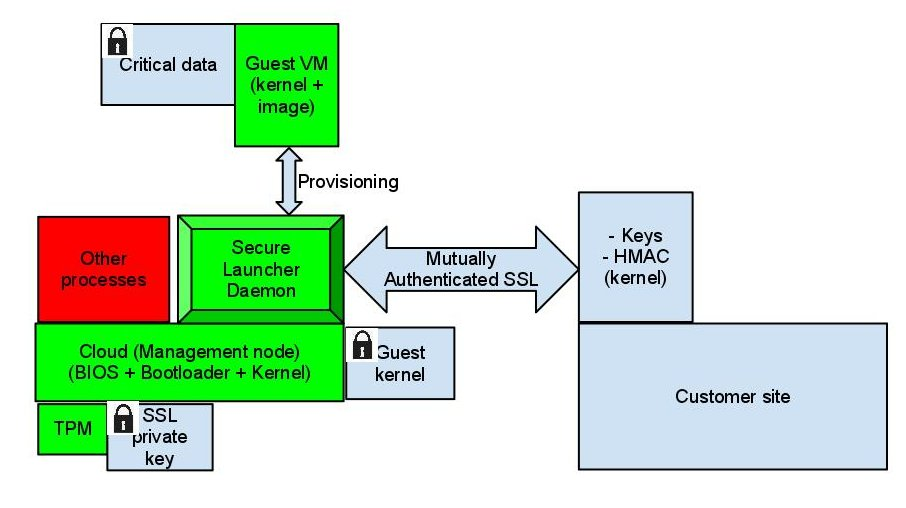
\includegraphics[scale=0.50]{csc574-solution.jpg}
\caption{\small \sl The architecture of the solution. The green parts denote trusted entities. Red denotes entities not in the TCB. The SSL private key is shown near the TPM block to signify that it is sealed in the TPM. The locked entities can only be unlocked by the trusted Secure Launcher Daemon. The guest VM resides on a different node. }
\label{fig:solution}
\end{figure*}
\subsection{Initial Setup}
For the success of this scheme, customer's participation is required in setting up the initial security of the system. In this section, we cover how the initial setup is done.

The customer first sets up separate keys for encryption/decryption of the kernel and the data. The cloud provider either sends a copy of the kernel to be authenticated by the customer or the customer compiles his own copy. In the former case, the unencrypted kernel is sent via snail-mail on a harddrive with proper digital signature. The customer verifies the digital signature, creates an HMAC with his kernel signing key and encrypts the kernel. The encrypted kernel is then returned via snail-mail, again, with proper digital signature. The customer keeps the HMAC. The cloud provider installs this encrypted kernel on his side. Note that the snail-mail is only to provide a secure out-of-band communication mechanism.

The customer then sets up an SSL-enabled server to serve the keys and the HMAC to properly authenticated cloud entity. 

On the cloud side, the customer takes part in setting up the TCB. The customer can, optionally, provide a TPM. The TPM setup procedure is fully audited by the customer to ensure security (Core assumption is that the cloud provider is trusted and the setup procedure won't be botched. The audit is to make sure that the proper security policies are adhered to). The setup of the management node occurs behind closed doors with no access to the external world, so it is assumed that it cannot be compromised by an external entity.

A proper hash of {BIOS, bootloader, kernel, secure launcher daemon} is extended in on the PCRs of the TPM. The SSL private key of the cloud used for authentication with the customer is then sealed off againt the said PCR. Proper SELinux policies are then put in place to sandbox the secure launcher daemon.

The next section describes the operation of the setup.

\subsection{Overview}
The very first step to secure data in the cloud is to encrypt it. The cloud provider can provide facilities for encryption just before storing to the persistent storage at the cloud site. However, according to the end-to-end argument \cite{end-to-end}, if the cloud customer needs guarantees, the encryption has to be done at the application layer by the customer software. The customer may choose to have a full-disk encryption (encrypts the whole filesystem) \cite{disk-encryption, truecrypt} or a selective file-encryption \cite{nss}. In either method, for efficiency reasons, the encryption technique chosen would probably be some kind of symmetric encryption (like AES) and will need a key. 

This key cannot be stored on the guest image in plaintext, since the attacker has access to the guest image from the management node and he can directly read it off the image. As describer above, the keys will be revealed only to a cloud process who can provide attestation (using TCB) and authenticate itself using SSL. Next we describe ways in which it will be impossible (or atleast hard) for an attacker to falsely pose to the customer as an attested cloud process.

Now refer to Figure \ref{fig:solution} for an overview of the architecture.
A TPM is used to establish a TCB, as we saw in the "Background" section. The TPM verifies the BIOS, bootloader and the kernel. Eventually, the kernel extends the hash of a \emph{secure launcher daemon} in the TPM and starts the daemon. The job of this daemon is to listen for requests to launch a VM. When a request is received, it unseals the SSL private key from the TPM. This unseal operation only works if neither of the BIOS, bootloader, kernel or secure launch daemon have been modified.

After the SSL private key is unsealed, the daemon can authenticate to the customer site. Once the customer site authenticates the cloud provider, it releases the following objects: kernel decryption key, data decryption key and an HMAC of the kernel image.

The \emph{secure launcher daemon} decrypts and verifies the integrity of the kernel. It then reads the actual launcher binary (usually a provisioning engine like xCAT \cite{xCAT}) into memory, calculates its hash and compares against the expected hash. If both the kernel and the launcher binary are verified, then the daemon forks of the launcher process which does the appropriate provisioning.

The data decryption keys are passed on to the guest kernel via a shared page or as a provisioning parameter.

Note that the \emph{secure launcher daemon} is confined using SELinux. The SELinux policy recommendations and how to sandbox the daemon is described in detail in a later section.

\section{Experimental Evaluation}
\label{sec:evaluation}


\section{Related work}
\label{sec:related}

\section{Conclusion}
\label{sec:conclusion}

\bibliography{references}{}
\bibliographystyle{plain}
\end{document}


